\section{Osculating Circles Estimator}

Osculating Circles Estimator (CC) is an algorithm that calculate the curvature of a contour, by pointing out the tangent circle at each point of the contour. 

\paragraph{}
For implementing this part, we used the definition of digital straight segment and digital straight line. 

\subsection{Digital Straight Line}
Digital Straight Line (DSL) is defined by 4 values : $D(a, b, \mu, \omega)$, with $a, b, c, d \in \mathbb{Z}$ and $gcd(a, b) = 1$. $a/b$ is called a sloped of $D$, $\mu$ is an intercept and $\omega$ is the thickness of $D$.

\paragraph{}
Every points that belong to $D(a, b, \mu, \omega)$ must satisfy :
$$
\mu \leq ax-by < \mu + \omega
$$

In DGtal, there are 2 types of DSL :
\begin{itemize}
\item Naive Digital Straight Line
\item Standard Digital Straight Line
\end{itemize}

These type of DSL is made by specifying the value \textit{thickness}. 

\begin{itemize}
\item Naive DSL : $\omega = max(|a|, |b|)$
\item Standard DSL : $\omega = |a| + |b|$
\end{itemize}

\subsection{Digital Straight Segment}
Digital Straight Segment (DSS) is the set of points that belong to a digital straight line. Just like DSL, in DGtal there are also two specifics DSS : Naive DSS and Standard DSS.

\subsection{Implementation}\FloatBarrier
In this project, we used the standard DSL and DSS to implement this algorithm. A class \textbf{ArithmeticalDSSComputer} will be used to analyze the points of the contour.
\begin{figure}[h]
    \centering
    \subfloat[Source File]{{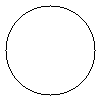
\includegraphics[width=5cm]{project/images/dsl_source.png} }}
    \qquad
    \subfloat[Result after applying the algorithm]{{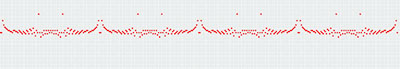
\includegraphics[width=5cm]{project/images/dsl_result.jpg} }}
    \caption{Source and Result}
    \label{fig:example}
\end{figure}
\paragraph{}
\textbf{StandardDSS4Computer} is the sub class of \textbf{ArithmeticalDSSComputer}, which is specialized which type of DSS that use to make the calculation. After extract all the points of the contour into a vector, we need to adjust this vector to be able to iterate through all the points of the contour. 

\paragraph{}
The idea of CC algorithm is that at each point of the contour, called K point, we will try to extend the DSS, which is started at the point we are at, to the utmost left (resp. utmost right). The last point that can be added to the DSS called L point (resp. R point). The three points K, L, R form a triangle. Call the rayon of the circle that go through these three points R. Then the curvature's value of point K will be :
$$
C(K) = \frac{sign(det(\overrightarrow{KR}, \overrightarrow{KL}))}{R}
$$.  
In case that these three points is alignment, the curvature's value is set to zero.

\paragraph{}
So the most important work in this algorithm, is to be able to locate the two points L and R with each point K that we iterate through. We need two DSS, one for searching the point R, another for searching the point L. In class \textbf{StandardDSS4Computer} there are two methods that could help with the searching : \textit{extendFront} and \textit{extendBack}. These two method will return true if they can still add point to the DSS, and false if not. So now the problem of searching for the two points L and R is solved. But we still have one more problem.

\paragraph{}
For calculating the curvature of point K, we have to have the two points L and R corresponded to the point K. So now what will happen if we are at the begin or the end of our vector ? Only one point, either L or R, could be found. The vector is the set of all the points of the contour, that means that the begining and the end of this vector, is at the same point of the contour. So the set of points obtained by \textit{StandardDSS4Computer::extendFront} at the begin of the vector, and the set of points obtained by \textit{StandardDSS4Computer::extendBack} at the end of the vector will be added to end and the head of the vector. Now, we can easily iterate through the set of points of the contour.

\subsection{Usage}
For testing this algorithm, go to the folder \textbf{TestDSL}, execute \textbf{cmake}, then \textbf{make}. Then run :\\
./TestDSL path-to-file \\
\textit{path-to-file} is a path to an image file, with \textbf{pgm} extention (Portable Graymap)





